\chapter{Metodologia e Sviluppo}
Di seguito, nel capitolo viene presentata l’architettura generale del sistema. Successivamente, l'implementazione dei diversi moduli della pipeline in MATLAB viene analizzata in dettaglio, con il supporto rappresentativo del paziente \textit{BRATS\_218.nii.gz}.

\section{Architettura della Pipeline di Elaborazione}
La pipeline è strutturata in fasi sequenziali, come illustrato in Figura~\ref{fig:pipeline}.

\begin{figure}[h]
    \centering
    \includesvg[width=\textwidth]{images/pipeline}
    \caption{Schema a blocchi della pipeline di segmentazione proposta.}
    \label{fig:pipeline}
\end{figure}

La pipeline si apre con una fase di analisi esplorativa (\textit{Exploratory Data Analysis}, EDA), finalizzata al confronto qualitativo delle diverse sequenze MRI mediante visualizzazione delle immagini, miglioramento del contrasto, rendering tridimensionale del volume e analisi degli istogrammi di intensità.

In seguito, le immagini sono sottoposte a una fase di pre-processing che include l’estrazione della slice più rilevante, la normalizzazione delle intensità, la riduzione del rumore con filtro mediano e costruzione di rappresentazioni multimodali. Viene, inoltre, generata la \textit{seed map}, utile per individuare la regione iniziale da cui avviare la segmentazione.

Quest'ultima è implementata mediante una strategia a cascata che combina più tecniche~\cite{peter2008}. Inizialmente, viene applicata una sogliatura multilivello basata sul metodo di Otsu per individuare le regioni di interesse. Successivamente, l'algoritmo \textit{Region Growing} espande tali regioni a partire dal seme e, infine, il \textit{Marker-Controlled Watershed} viene impiegato per migliorare la maschera di segmentazione ottenuta.

Al termine del processo, tali maschere vengono rifinite attraverso una fase di post-processing basata su operazioni morfologiche per riempire eventuali lacune e rimuovere componenti connesse non necessarie.

Infine, le prestazioni della pipeline sono valutate mediante un confronto tra le maschere predette e le corrispondenti ground truth binarie, utilizzando metriche standard quali Dice Score, \textit{Precision} e Sensitivity.

\section{Implementazione in MATLAB}
Per l'implementazione in ambiente MATLAB, sono state utilizzate le funzionalità offerte dall’\textit{Image Processing Toolbox}~\cite{matlab2025b}. Inoltre, il progetto è stato organizzato secondo una struttura modulare in funzioni, per separare le fasi di elaborazione.

All’interno della cartella principale del progetto sono presenti le sottocartelle relative alla gestione dei dati e dei risultati. La cartella \textit{/dataset} contiene i volumi MRI in formato NIfTI per tutti i pazienti considerati e le corrispondenti ground truth. La cartella \textit{/results} è, invece, destinata al salvataggio dei risultati. Per ciascun paziente, la pipeline salva le figure relative alle sequenze originali, agli step di pre-processing, ai risultati intermedi della segmentazione, al post-processing e al confronto finale con la ground truth.

\subsection{Script Principale (Main)}
Il file \textit{main.m} costituisce il punto di ingresso dell’intera pipeline e gestisce il caricamento dei dati, il richiamo sequenziale dei moduli di pre-processing, segmentazione, valutazione e la generazione dei risultati grafici e numerici.

\paragraph{Caricamento dei file}
Lo script definisce i percorsi delle cartelle contenenti i volumi MRI e le relative ground truth.

Mediante la funzione \textit{dir} vengono individuati tutti i file con estensione \textit{.nii.gz} presenti nella cartella delle immagini, ottenendo l’elenco completo dei pazienti da elaborare. Il numero totale dei file viene memorizzato nella variabile \textit{num\_files}.

Prima di avviare l’elaborazione, viene inizializzato un array di struct denominato \textit{metrics}, con dimensione pari al numero di pazienti. Ogni elemento della struttura contiene il nome del paziente e le metriche di valutazione associate alle cinque configurazioni sperimentali (\textit{FLAIR}, \textit{T1c}, \textit{T2}, \textit{Fusion2} e \textit{Fusion3}).

\paragraph{Elaborazione iterativa}
Mediante un un ciclo \textit{for} che itera su tutti i pazienti del dataset, vengono definiti il nome del file corrente, i percorsi specifici dell’immagine e della ground truth e la cartella di output dedicata al paziente.

Per ciascun paziente, lo script richiama in sequenza la funzione \textit{pre\_processing}, che restituisce le immagini preprocessate delle diverse sequenze, le fusioni multimodali, la maschera di ground truth della slice selezionata e la \textit{seed map} per l'avvio della segmentazione. Inoltre, con chiamate ripetute alla funzione \textit{segmentation}, si ottengono le maschere di segmentazione post-processate per ciascuna delle configurazioni. Successivamente, attraverso la funzione \textit{evaluation}, ciascuna maschera predetta viene confrontata con la ground truth e vengono calcolate le metriche di valutazione, poi salvate nella struttura \textit{metrics} aggiornando i campi relativi al paziente corrente.

\paragraph{Generazione dei risultati}
Per ciascun paziente viene costruita una figura (\textit{comparison\_results.png}) composta da sei subplot disposti su una griglia \(2 \times 3\). Nel primo pannello viene visualizzata la ground truth con immagine \textit{T1} di sfondo, mentre nei cinque pannelli successivi vengono mostrate le segmentazioni ottenute dalle diverse configurazioni con il contorno della ground truth in verde e quello della segmentazione in rosso.

Durante l’esecuzione, lo script stampa nella Command Window una riga di avanzamento per ogni paziente, riportando il numero progressivo del caso e i valori di \textit{Dice Score} ottenuti per tutte le configurazioni considerate.

Al termine dell’elaborazione, viene stampato il riepilogo delle metriche medie e vengono prodotti due file \textit{CSV}. Il primo, \textit{detailed.csv}, contiene una riga per ciascun paziente e riporta tutte le metriche ottenute per ogni configurazioni. Il secondo, \textit{global.csv}, contiene invece i valori medi delle metriche calcolate sull’intero dataset per ciascuna sequenza.

\subsection{Analisi Esplorativa dei Dati (EDA)}
La fase di EDA consente di confrontare il comportamento delle diverse sequenze MRI, analizzandone sia l’aspetto visivo sia la distribuzione delle intensità prima e dopo il miglioramento del contrasto.

\paragraph{Caricamento dei dati}
Inizialmente, viene selezionato il paziente desiderato e vengono definiti i percorsi del volume MRI e della ground truth in formato NIfTI. Inoltre, viene creata la cartella per il salvataggio delle figure prodotte durante l’analisi.

Successivamente, vengono letti i volumi con la funzione \textit{niftiread} e convertiti in formato \textit{double}, per facilitare le operazioni successive.

L'analisi è effettuata in modo semplificato sulla slice centrale del volume, la numero 78. Nella pipeline completa, invece, la selezione della slice avviene in modo automatico, individuando quella con maggiore estensione della regione tumorale.

\paragraph{Visualizzazione delle sequenze originali}
A partire dalla sequenza \textit{FLAIR}, viene costruita una maschera cerebrale binaria per limitare l’analisi ai soli pixel appartenenti al cervello, escludendo lo sfondo nero che altererebbe la distribuzione delle intensità.

Lo script genera una figura contenente, nella riga superiore, la visualizzazione delle quattro sequenze originali e, nella riga inferiore, i corrispondenti istogrammi delle intensità all’interno della regione cerebrale. Per la visualizzazione delle immagini viene utilizzata la funzione \textit{mat2gray}, che rimappa i valori nell’intervallo $[0,1]$, come illustrato in Figura~\ref{fig:eda_raw_sequences}.

\begin{figure}[H]
    \centering
    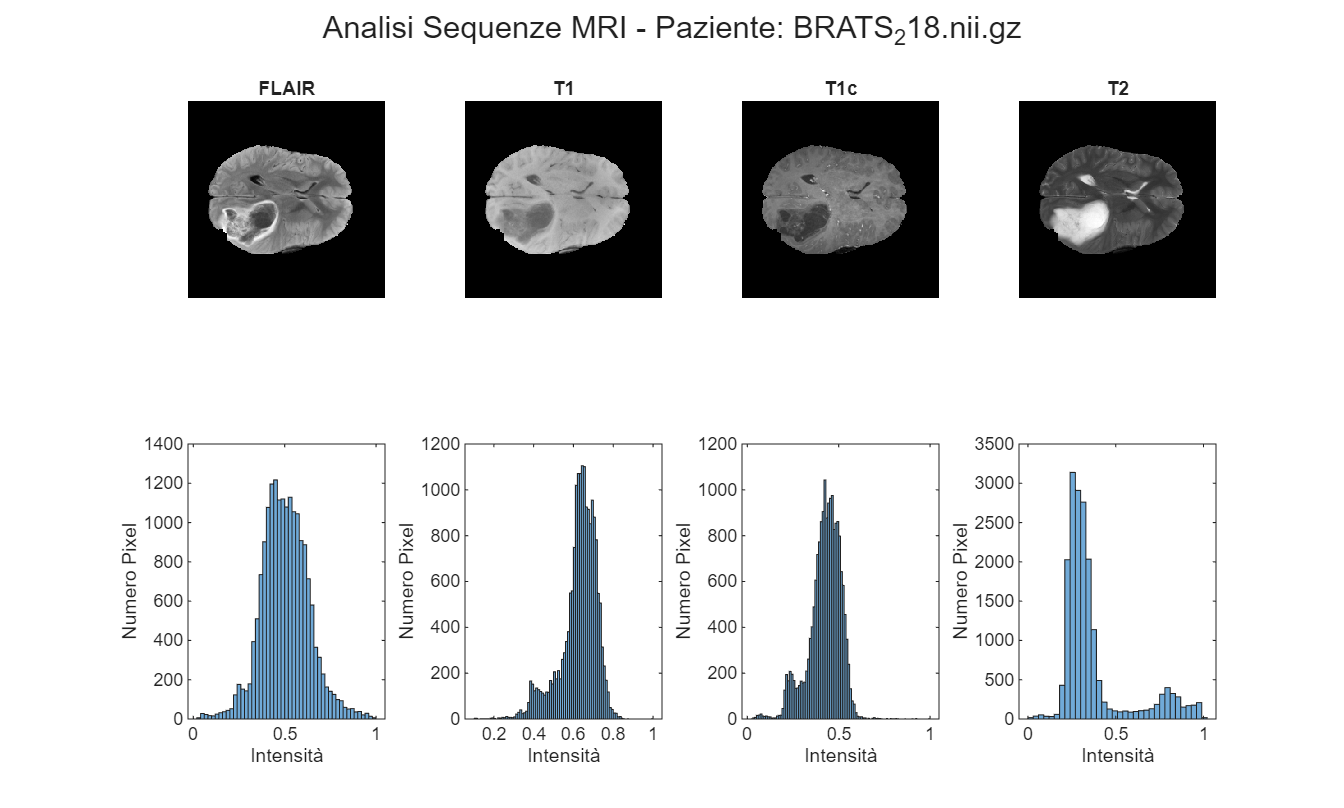
\includegraphics[width=\textwidth]{images/218_Raw_sequences.png}
    \caption{Analisi delle sequenze MRI originali per le immagini \textit{FLAIR}, \textit{T1}, \textit{T1c} e \textit{T2} estratte dalla slice selezionata e i relativi istogrammi delle intensità nella regione cerebrale.}
    \label{fig:eda_raw_sequences}
\end{figure}

\paragraph{Miglioramento del contrasto con CLAHE}
Per migliorare la visualizzazione, per ciascuna sequenza è stata applicata la tecnica di \textit{Contrast Limited Adaptive Histogram Equalization} (CLAHE), implementata tramite la funzione \textit{adapthisteq}. Nel codice è stato impostato il parametro \textit{ClipLimit = 0.015}, che controlla la soglia massima dei livelli di intensità per ciascun blocco dell’immagine, limitando i picchi più elevati e redistribuendo uniformemente l'eccesso sugli altri livelli. La Figura~\ref{fig:eda_clahe_sequences} mostra le immagini dopo l’enhancement e gli istogrammi corrispondenti.

\begin{figure}[H]
    \centering
    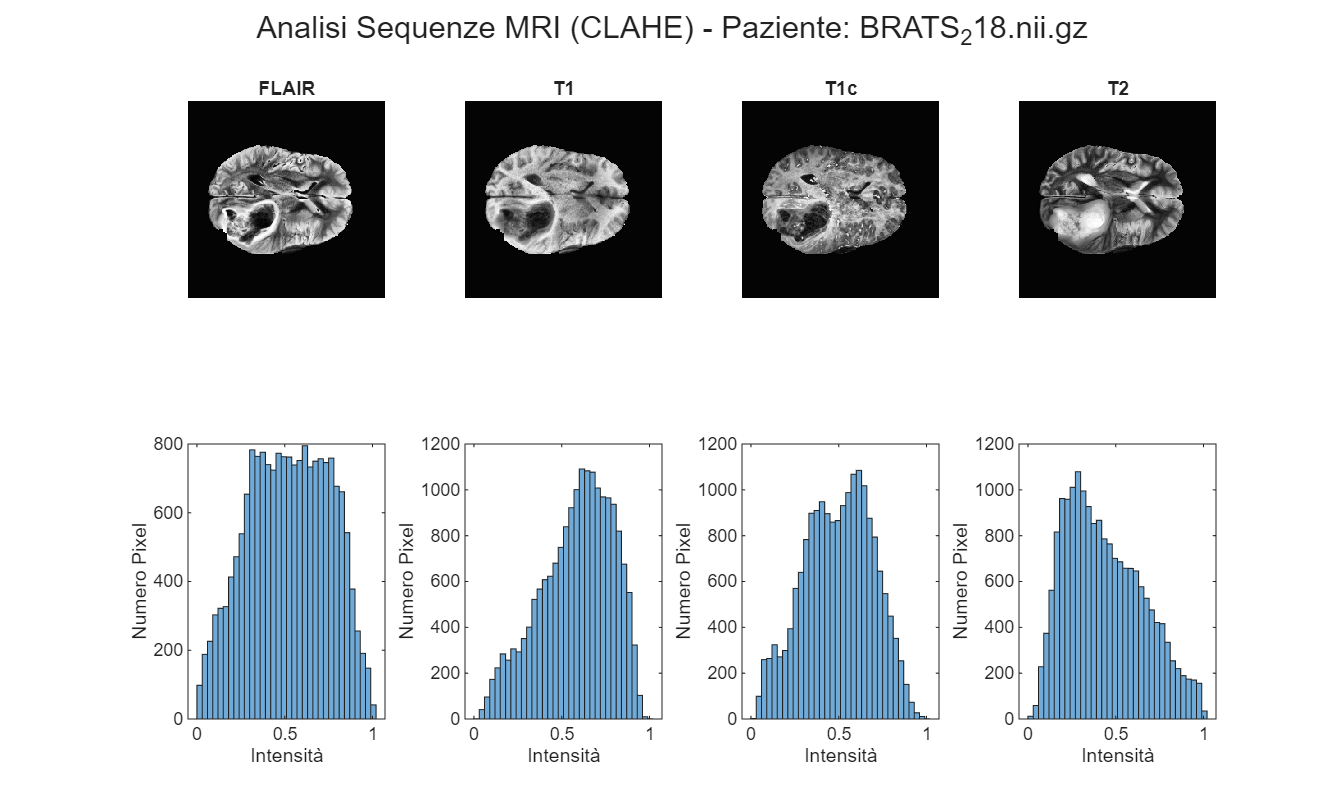
\includegraphics[width=\textwidth]{images/218_CLAHE_sequences.png}
    \caption{Analisi delle sequenze MRI dopo miglioramento del contrasto mediante CLAHE per le immagini e le rispettive distribuzioni di intensità.}
    \label{fig:eda_clahe_sequences}
\end{figure}

\paragraph{Visualizzazione volume 3D}
Infine, lo script utilizza la funzione \textit{volshow} per visualizzare interattivamente il volume tridimensionale della sequenza \textit{FLAIR}, come mostrato in Figura~\ref{fig:3d_eda}.

\begin{figure}[H]
    \centering
    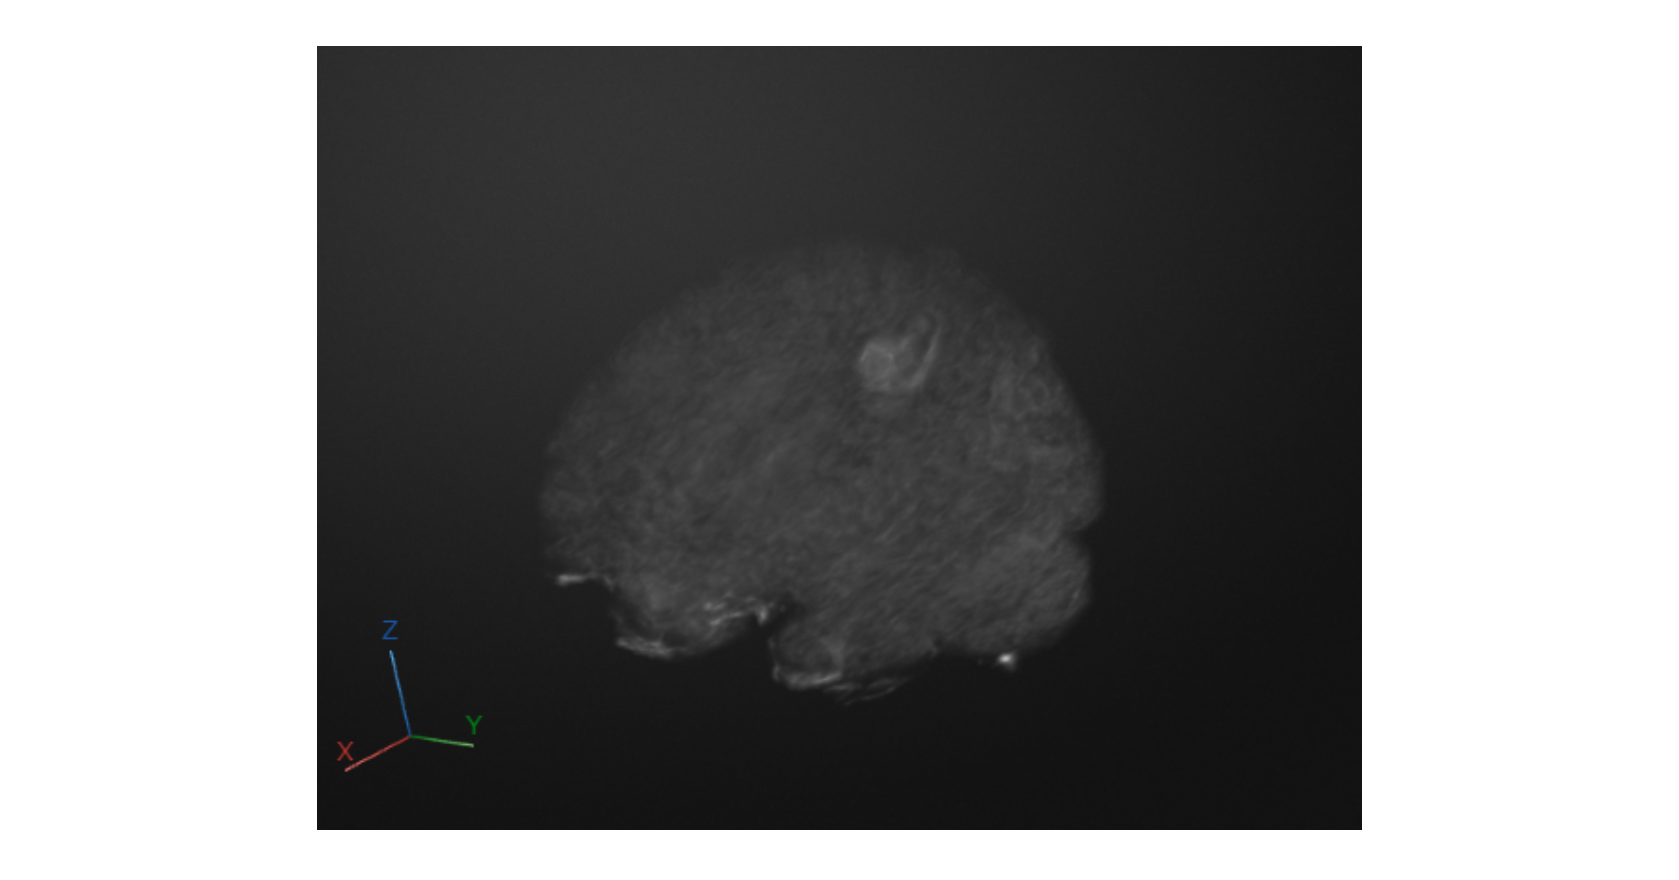
\includegraphics[width=\textwidth]{images/eda_3d_volume.png}
    \caption{Rendering tridimensionale interattivo della sequenza \textit{FLAIR} per l’analisi qualitativa della struttura cerebrale.}
    \label{fig:3d_eda}
\end{figure}

\subsection{Pre-Processing}
La fase di pre-processing ha il compito di trasformare i dati grezzi estratti dal dataset in immagini adeguate per la segmentazione.

\paragraph{Selezione automatica della slice più rilevante}
All'inizio, vengono caricati il volume MRI e la relativa ground truth tramite la funzione \textit{niftiread}, poi convertiti in formato \textit{double}. A differenza di quanto descritto per la fase di EDA, viene individuata automaticamente la slice più significativa calcolando, per ognuna di esse, il numero di pixel appartenenti alla regione tumorale nella ground truth e selezionando quella che presenta la massima estensione della lesione.

Detta $G(x,y,z)$ la ground truth binaria tridimensionale, lo score associato alla slice $z$ è definito come:
\[
s(z) = \sum_{x}\sum_{y} \mathbf{1}\big(G(x,y,z)>0\big)
\]
La slice scelta corrisponde quindi a:
\[
z_{\text{best}} = \arg\max_{z} s(z)
\]

Identificata tale slice, da essa vengono estratte le sequenze \textit{FLAIR}, \textit{T1}, \textit{T1c}, \textit{T2} e le maschere di ground truth corrispondenti.

\paragraph{Costruzione della maschera cerebrale}
La maschera cerebrale della regione di interesse (ROI) viene costruita a partire dalla sequenza \textit{FLAIR}, selezionando i pixel con intensità positiva e applicando l’operazione \textit{imfill} per riempire eventuali lacune interne.

\paragraph{Analisi delle sequenze grezze}
Il codice genera una figura contenente le sequenze grezze e i relativi istogrammi delle intensità nella regione cerebrale per la sola slice ottimale individuata, come riportato in Figura~\ref{fig:pre_raw_histogram}.

\begin{figure}[H]
    \centering
    \includegraphics[width=\textwidth]{images/218_Raw_histogram.png}
    \caption{Sequenze MRI grezze estratte dalla slice ottimale, con i relativi istogrammi delle intensità calcolati nella ROI cerebrale.}
    \label{fig:pre_raw_histogram}
\end{figure}

\paragraph{Normalizzazione delle intensità}
La normalizzazione viene applicata ai pixel interni alla maschera mediante trasformazione Z-score.
Per una generica immagine $I$, la normalizzazione è definita come:
\[
I_{\text{norm}}(x,y) = \frac{I(x,y)-\mu_I}{\sigma_I}
\]
dove $\mu_I$ e $\sigma_I$ rappresentano, rispettivamente, la media e la deviazione standard delle intensità.

Nel codice, questa operazione viene applicata a tutte le sequenze. Tuttavia, soltanto le sequenze \textit{FLAIR}, \textit{T1c} e \textit{T2} vengono poi impiegate nella costruzione delle fusioni multimodali, mentre la \textit{T1} viene mantenuta come riferimento visivo. Dopo la normalizzazione, i pixel esterni alla maschera cerebrale vengono azzerati per sopprimere lo sfondo e le sequenze vengono traslate nell’intervallo $[0,1]$ con la funzione \textit{mat2gray}.

\paragraph{Riduzione del rumore}
Per attenuare il rumore preservando i contorni delle strutture anatomiche, viene applicato un filtro mediano bidimensionale con kernel $3\times3$, implementato tramite la funzione \textit{medfilt2}. Il filtro mediano è un operatore non lineare adatto alla rimozione di rumore impulsivo, che sostituisce il valore di ciascun pixel con la mediana dei valori presenti nel suo intorno locale.

Le Figure~\ref{fig:pre_flair}, \ref{fig:pre_t1c} e \ref{fig:pre_t2} mostrano i principali step del pre-processing (sequenza grezza, normalizzata e filtrata), insieme agli istogrammi delle intensità.

\begin{figure}[H]
    \centering
    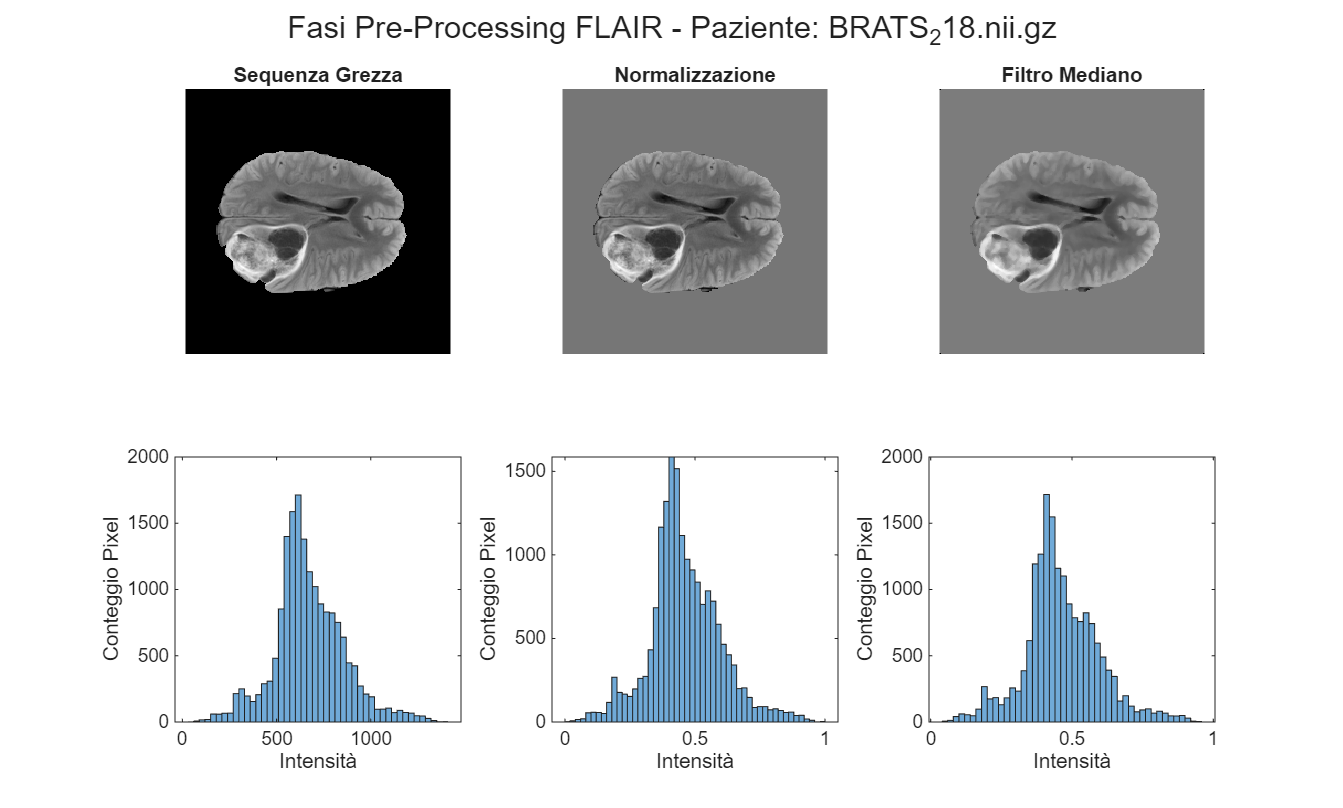
\includegraphics[width=\textwidth]{images/218_FLAIR_pre_processing.png}
    \caption{Fasi di pre-processing della sequenza \textit{FLAIR}: immagine grezza, normalizzazione delle intensità e filtraggio mediano, con i rispettivi istogrammi.}
    \label{fig:pre_flair}
\end{figure}

\begin{figure}[H]
    \centering
    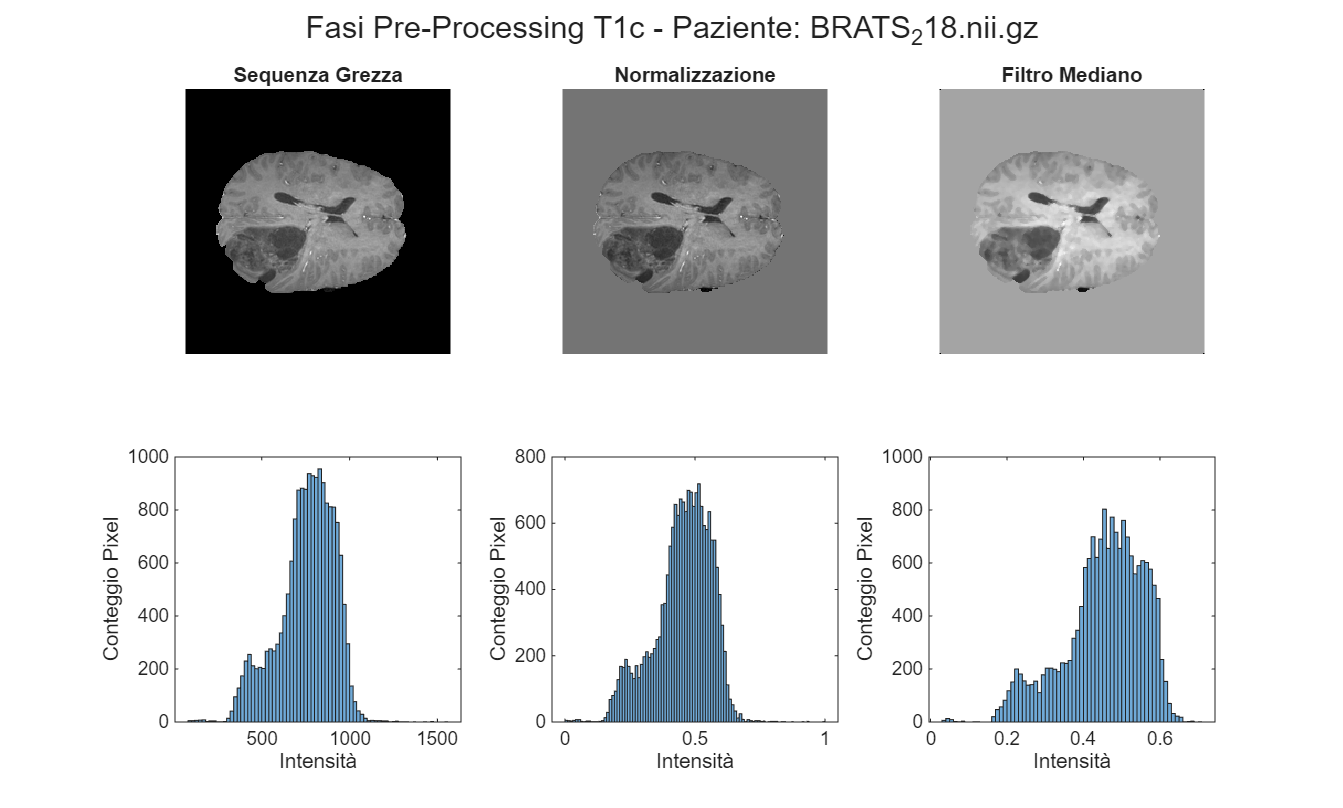
\includegraphics[width=\textwidth]{images/218_T1c_pre_processing.png}
    \caption{Fasi di pre-processing della sequenza \textit{T1c}: immagine grezza, normalizzazione delle intensità e filtraggio mediano, con i rispettivi istogrammi.}
    \label{fig:pre_t1c}
\end{figure}

\begin{figure}[H]
    \centering
    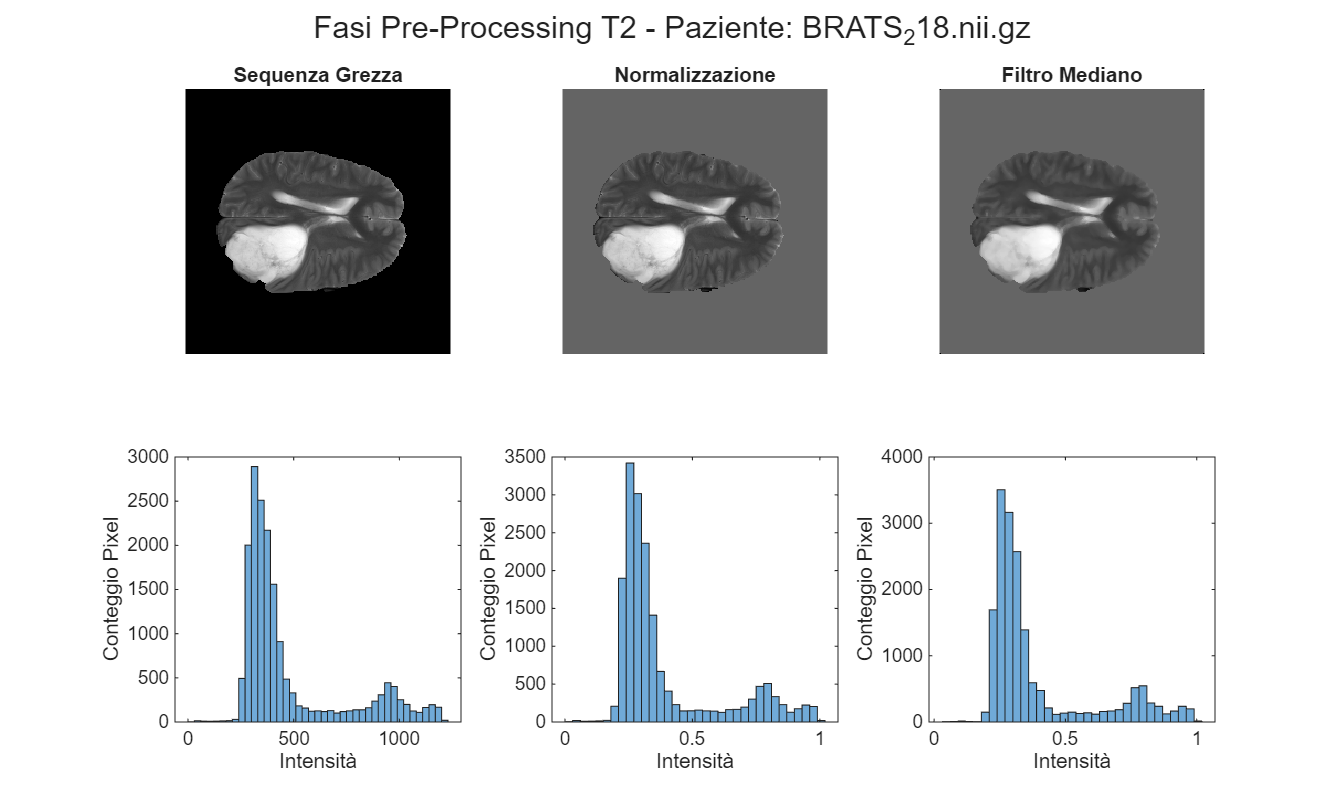
\includegraphics[width=\textwidth]{images/218_T2_pre_processing.png}
    \caption{Fasi di pre-processing della sequenza \textit{T2}: immagine grezza, normalizzazione delle intensità e filtraggio mediano, con i rispettivi istogrammi.}
    \label{fig:pre_t2}
\end{figure}

\paragraph{Costruzione delle rappresentazioni multimodali}
Nel codice vengono costruite due configurazioni di fusione secondo una combinazione lineare pesata:
\[
I_{\text{Fusion2}} = 0.6\,I_{\text{FLAIR}} + 0.4\,I_{\text{T1c}}
\]
\[
I_{\text{Fusion3}} = 0.5\,I_{\text{FLAIR}} + 0.2\,I_{\text{T1c}} + 0.3\,I_{\text{T2}}
\]

La prima configurazione, denominata \textit{Fusion2}, integra l’informazione proveniente da \textit{FLAIR} e \textit{T1c}, mentre la seconda, \textit{Fusion3}, include anche il contributo della sequenza \textit{T2}. I pesi sono stati scelti empiricamente, attribuendo maggiore importanza alla modalità \textit{FLAIR}, poiché rappresentativa dell’estensione complessiva della lesione, ma mantenendo un contributo complementare per \textit{T1c} e \textit{T2}.

Le Figure~\ref{fig:pre_fusion2} e \ref{fig:pre_fusion3} mostrano il risultato di tali combinazioni e i corrispondenti istogrammi delle intensità.

\begin{figure}[H]
    \centering
    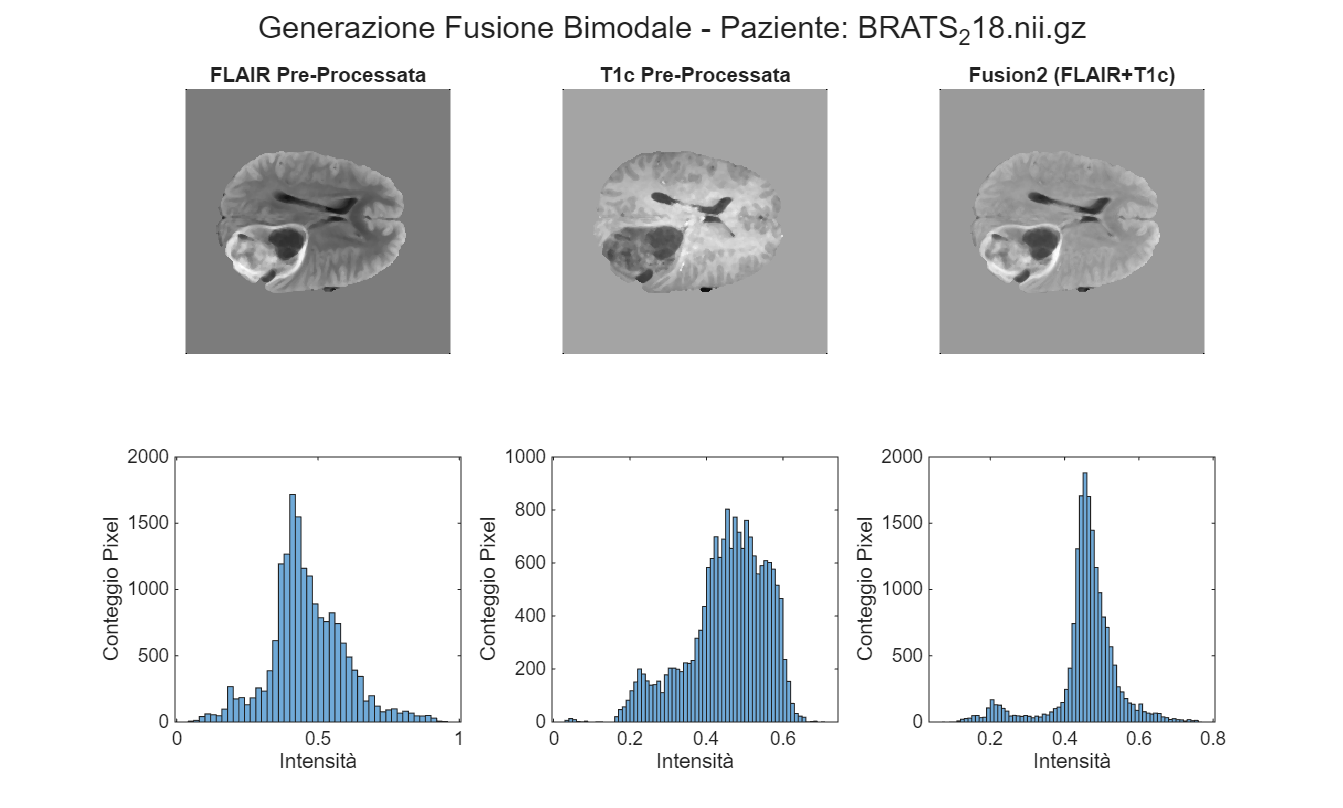
\includegraphics[width=\textwidth]{images/218_Fusion2_pre_processing.png}
    \caption{Generazione della fusione bimodale a partire dalle sequenze \textit{FLAIR} e \textit{T1c} pre-processate, con i corrispondenti istogrammi delle intensità.}
    \label{fig:pre_fusion2}
\end{figure}

\begin{figure}[H]
    \centering
    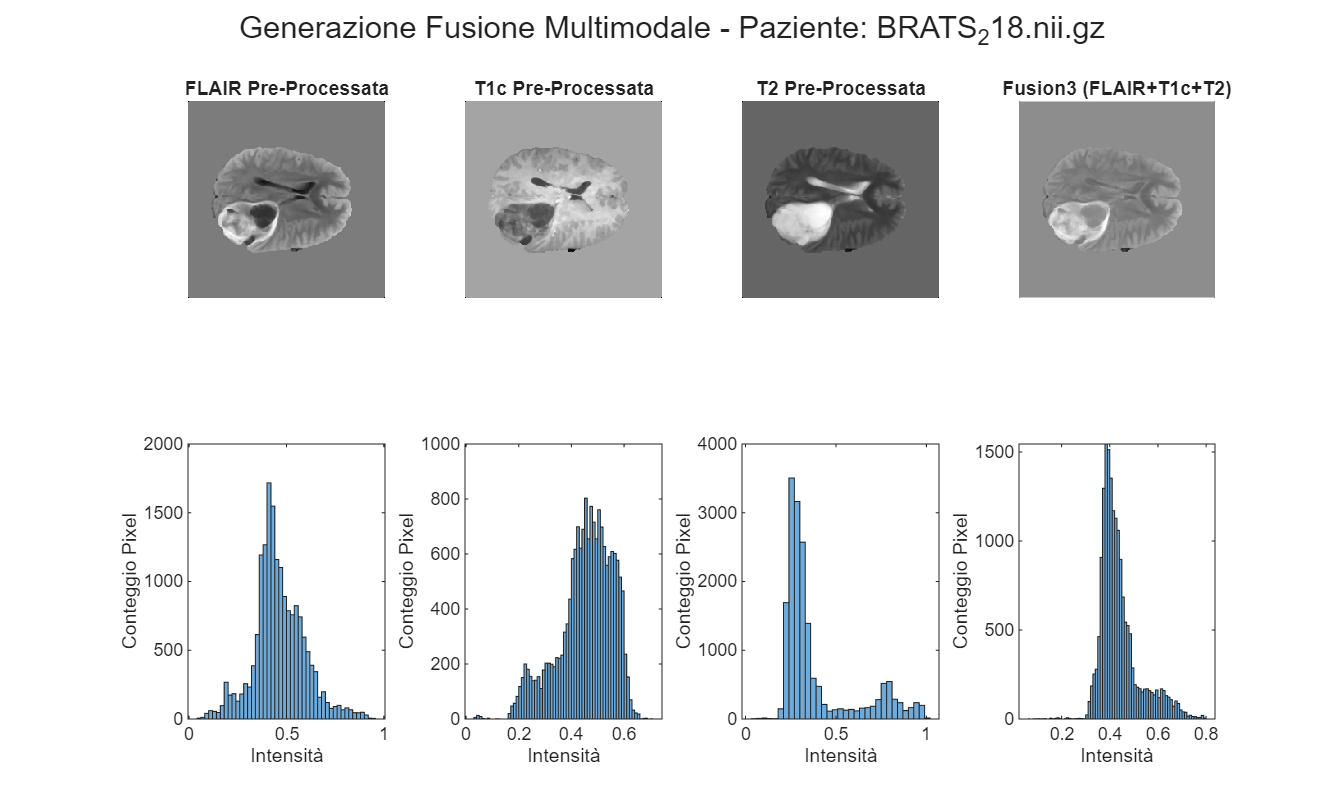
\includegraphics[width=\textwidth]{images/218_Fusion3_pre_processing.png}
    \caption{Generazione della fusione multimodale a partire dalle sequenze \textit{FLAIR}, \textit{T1c} e \textit{T2} pre-processate, con i corrispondenti istogrammi delle intensità.}
    \label{fig:pre_fusion3}
\end{figure}

\paragraph{Generazione della seed map}
La \textit{seed map} in Figura~\ref{fig:pre_seed_map} è stata ottenuta applicando un filtro gaussiano alla rappresentazione \textit{Fusion3} tramite la funzione \textit{imgaussfilt} con parametro $\sigma = 3$. A differenza del filtro mediano, impiegato per la riduzione del rumore locale, il filtro gaussiano introduce una sfocatura controllata per smussare le variazioni locali e far emergere la regione a intensità globale più elevata.
Il valore di $\sigma$ non è stato fissato manualmente, ma scelto sperimentalmente valutando l’andamento del \textit{Dice Score} medio al variare del livello di sfocatura gaussiana, come mostrato in Figura~\ref{fig:sigma_dice}.

\begin{figure}[H]
    \centering
    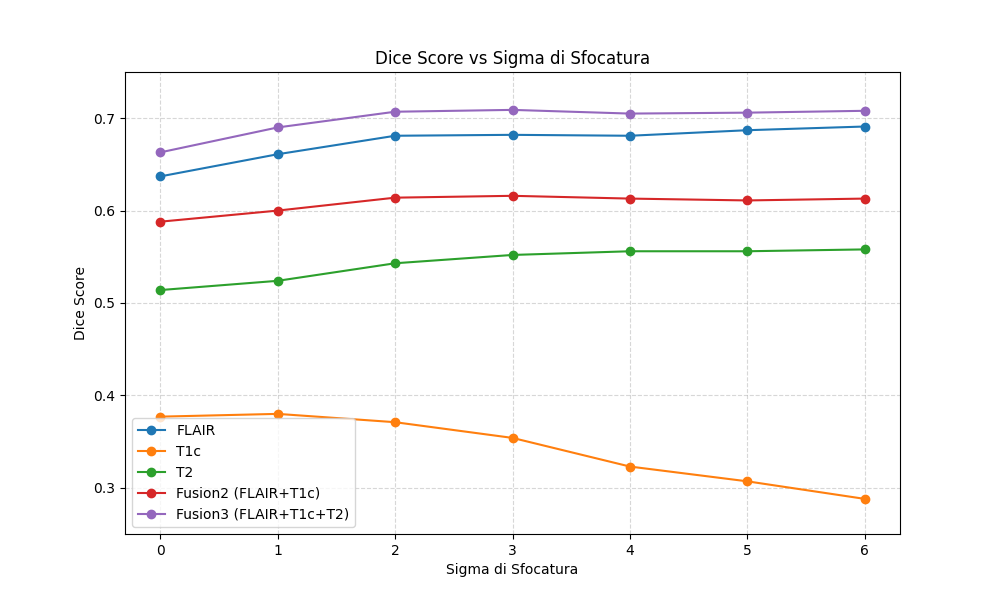
\includegraphics[width=0.82\textwidth]{images/sigma_dice.png}
    \caption{Andamento del \textit{Dice Score} medio al variare del parametro di sfocatura gaussiana $\sigma$ utilizzato per la generazione della \textit{seed map}.}
    \label{fig:sigma_dice}
\end{figure}

\begin{figure}[H]
    \centering
    \includegraphics[width=0.72\textwidth]{images/218_Seed_map.png}
    \caption{Seed map ottenuta applicando una sfocatura gaussiana alla rappresentazione \textit{Fusion3}.}
    \label{fig:pre_seed_map}
\end{figure}

\subsection{Segmentazione}
La fase principale di segmentazione è implementata nel modulo \textit{segmentation.m}. L’obiettivo è ottenere una maschera binaria che identifichi la regione tumorale nelle immagini pre-processate mediante una strategia a cascata, che combina le tre tecniche classiche di \textit{Image Processing} presentate in precedenza.

L’idea alla base della pipeline è combinare in modo complementare i diversi algoritmi, così da ottenere una prima regione di interesse, espanderla a partire da un seme interno e rifinirne progressivamente i contorni.

\paragraph{Selezione automatica del seme}
Prima di avviare la segmentazione, si individua automaticamente il seme iniziale sfruttando la seed map generata nella fase di pre-processing.
In particolare, viene identificato il pixel corrispondente al massimo della mappa:
\[
(x_{\text{seed}}, y_{\text{seed}}) = \arg\max_{(x,y)} \textit{SeedMap}(x,y)
\]

\paragraph{Otsu multilivello}
Il primo passo della segmentazione consiste nella sogliatura multilivello basata sul metodo di Otsu~\cite{otsu1979}. Tale approccio determina una o più soglie di intensità massimizzando la varianza inter-classe e minimizzando la varianza intra-classe tra i livelli di grigio. Il metodo opera direttamente sull’istogramma dei livelli di grigio dell’immagine, ricercando la soglia che suddivide i pixel in classi omogenee al loro interno ma il più possibile separate tra loro.

Nel lavoro viene utilizzata una sogliatura a due livelli, ottenuta tramite la funzione \textit{multithresh}, che suddivide l’immagine in tre classi di intensità. La maschera iniziale viene poi costruita selezionando i pixel appartenenti alla classe a intensità più elevata:
\[
M_{\text{Otsu}}(x,y)=
\begin{cases}
1 & \text{se } I(x,y) > T_2 \\
0 & \text{altrimenti}
\end{cases}
\]
dove $T_2$ rappresenta la soglia più alta restituita da Otsu.

\paragraph{Region Growing con seme automatico}
A partire dal seme selezionato, viene applicato un algoritmo di Region Growing, implementato nella funzione \textit{region\_growing.m}. Tale tecnica segmenta l’immagine espandendo iterativamente una regione iniziale verso i pixel adiacenti che soddisfano un opportuno criterio di omogeneità~\cite{adams1994}.

Un punto viene aggiunto alla regione se la sua intensità supera una determinata soglia calcolata a partire dalla maschera di Otsu.
Tale soglia viene scelta come il 6\textsuperscript{o} percentile delle intensità dei pixel appartenenti a $M_{\text{Otsu}}$:
\[
T_{\text{RG}} = \operatorname{percentile}_{6}\big(I(x,y)\;|\;M_{\text{Otsu}}(x,y)=1\big)
\]

Dunque, si considerano tutte le intensità dei pixel nella maschera, si ordinano in senso crescente e si seleziona il valore al di sotto del quale cade il 6\% dei campioni. L’utilizzo del un percentile rende il metodo dinamico rispetto alla distribuzione delle intensità del singolo paziente. Il valore corrispondente è individuato empiricamente, confrontando i risultati di \textit{Dice Score} al variare del percentile, come illustrato in Figura~\ref{fig:percentile_dice}.

\begin{figure}[H]
    \centering
    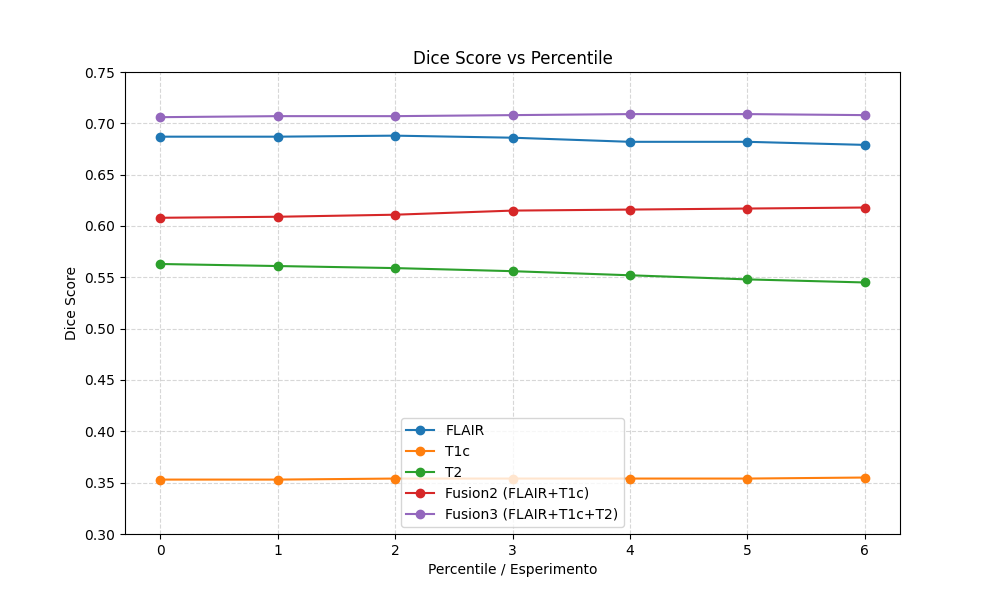
\includegraphics[width=0.82\textwidth]{images/percentile_dice.png}
    \caption{Andamento del \textit{Dice Score} medio al variare del percentile utilizzato per definire la soglia del Region Growing.}
    \label{fig:percentile_dice}
\end{figure}

L’espansione viene effettuata considerando un intorno a 8-connettività, che include non solo i quattro vicini ortogonali, ma anche i quattro vicini diagonali, garantendo una crescita continua della regione tumorale e riducendo la frammentazione.

Dal punto di vista implementativo, la funzione \textit{region\_growing.m} riceve in ingresso l’immagine $I$, le coordinate del seme iniziale $(seedY, seedX)$ e la soglia di intensità $T_{\text{RG}}$ e costruisce progressivamente una maschera binaria (\textit{mask}), inizialmente vuota, e una mappa (\textit{visited}) che tiene traccia dei pixel già esaminati.

Per gestire l’esplorazione è utilizzata una coda, realizzata con due vettori \textit{Q\_row} e \textit{Q\_col}, che memorizzano le coordinate di riga e colonna dei pixel da visitare. Il seed iniziale viene inserito in coda, marcato come visitato e incluso nella maschera finale.

Successivamente, l’algoritmo esegue le iterazioni finché la coda non risulta vuota. A ogni iterazione viene estratto il pixel corrente dalla testa della coda e vengono analizzati gli 8 vicini. Per ciascun vicino, si verifica che gli indici non eccedano i limiti dell’immagine e si controlla se il pixel è già stato visitato.

In caso negativo, esso viene segnato come visitato e, se la sua intensità risulta superiore alla soglia \textit{thresh}, il pixel viene aggiunto alla regione segmentata e accodato. Diversamente, il pixel viene escluso dalla regione.

\paragraph{Watershed con marcatori}
La maschera prodotta dal \textit{Region Growing} viene migliorata mediante l’algoritmo Marker-Controlled Watershed~\cite{vincent1991}, che considera l’immagine come una superficie topografica e separa le regioni in base alle zone che si sviluppano attorno agli stessi minimi locali. 

Tuttavia può soffrire di \textit{over-segmentation}, generando un numero elevato di regioni piccole e sparse. Per ridurre questo effetto, sono stati impiegati marcatori espliciti estratti dal Region Growing~\cite{grau2004}.
In particolare, viene calcolata la trasformata della distanza inversa sulla maschera ottenuta da esso:
\[
D = -\,\operatorname{bwdist}(\neg M_{\text{RG}})
\]
dove $\operatorname{bwdist}$ rappresenta la distanza euclidea e $\neg M_{\text{RG}}$ indica i pixel esterni alla maschera. Successivamente, i minimi locali della superficie vengono imposti utilizzando la maschera di Otsu come marker:
\[
D_{\text{mod}} = \operatorname{imimposemin}(D, M_{\text{Otsu}})
\]

Per evitare l’espansione verso lo sfondo, la trasformata viene limitata ponendo a $-\infty$ i valori esterni all'area considerata. Infine, i bordi di separazione ottenuti vengono rimossi e viene selezionata esclusivamente la componente connessa contenente il seme iniziale, ovvero la regione tumorale.

\paragraph{Risultati intermedi della segmentazione}
Per ciascuna configurazione analizzata, viena salvata una figura che riassume i passaggi della pipeline, tra cui la maschera ottenuta con Otsu (in giallo), l'espansione del \textit{Region Growing} (in ciano), il risultato del Watershed (in magenta) e la maschera finale non rifinita (in rosso), come riportato di seguito.

\begin{figure}[H]
    \centering
    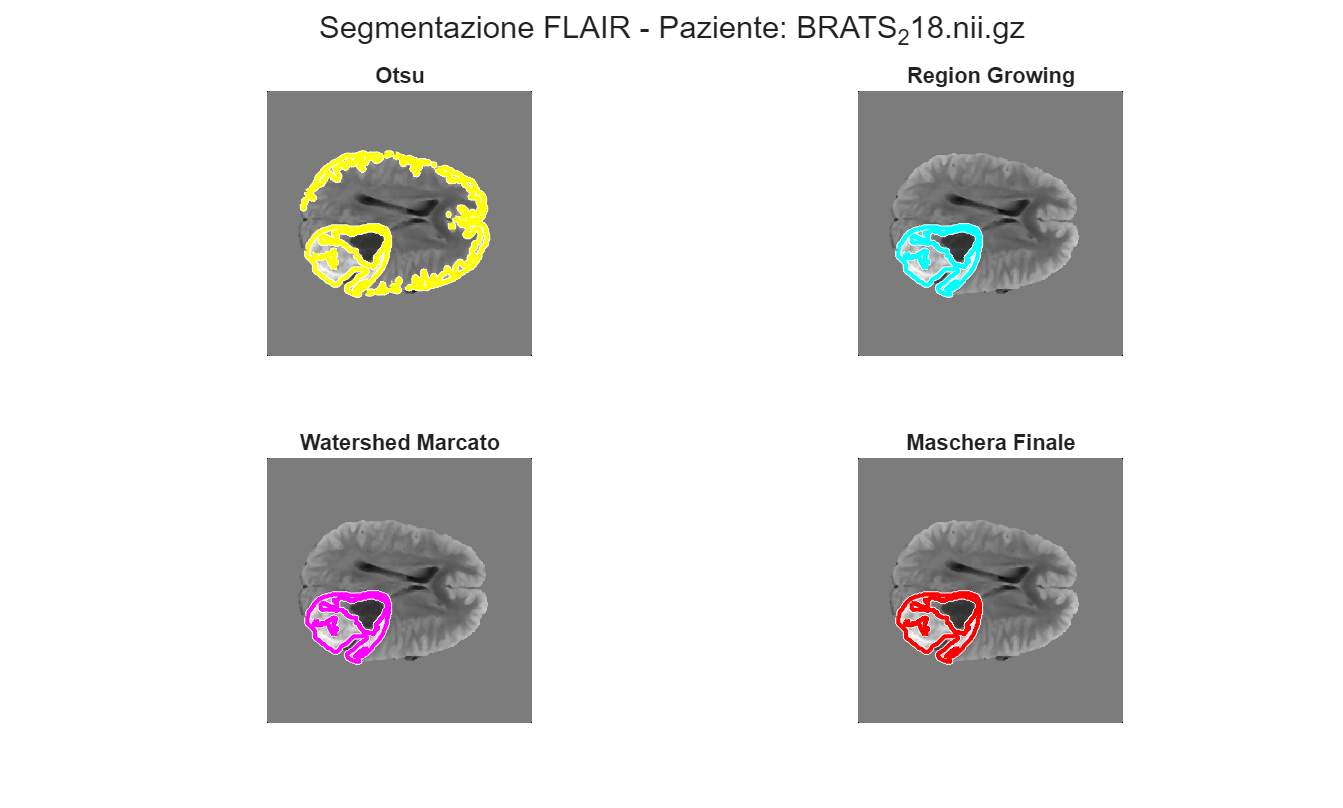
\includegraphics[width=\textwidth]{images/218_FLAIR_segmentation.png}
    \caption{Risultati intermedi della segmentazione sulla sequenza \textit{FLAIR}.}
    \label{fig:seg_flair}
\end{figure}

Nella Figura~\ref{fig:seg_flair}, la segmentazione iniziale ottenuta con Otsu risulta ampia e con regioni spurie lungo la periferia cerebrale. Il \textit{Region Growing} consente di selezionare la componente connessa più pertinente attorno al seme, mentre il \textit{Marker-Controlled Watershed} ne rifinisce il contorno.

\begin{figure}[H]
    \centering
    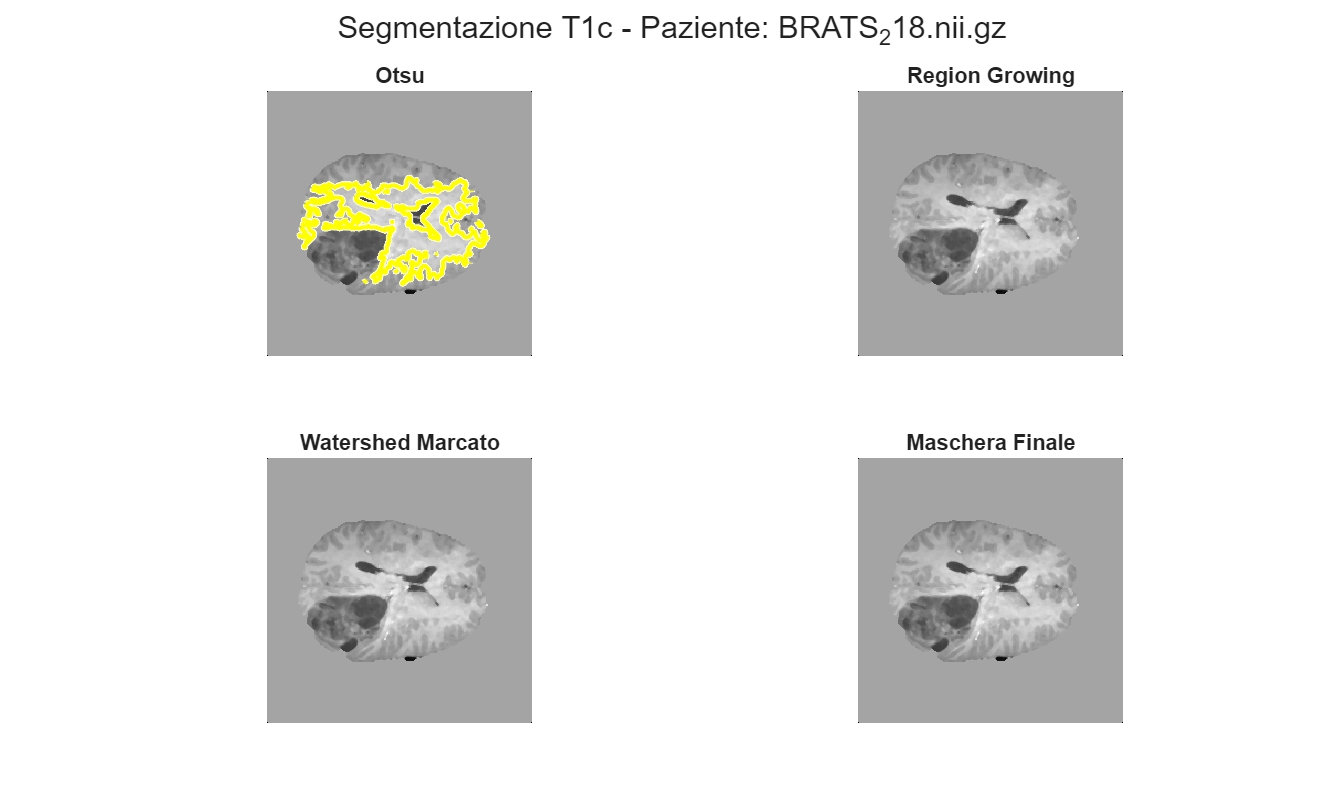
\includegraphics[width=\textwidth]{images/218_T1c_segmentation.png}
    \caption{Risultati intermedi della segmentazione sulla sequenza \textit{T1c}.}
    \label{fig:seg_t1c}
\end{figure}

Nel caso della sequenza \textit{T1c} in Figura~\ref{fig:seg_t1c}, la sogliatura di Otsu individua diverse regioni ad alta intensità distribuite nell’immagine, che non risultano sufficientemente connesse con l’intera estensione della lesione. Di conseguenza, le successive fasi di \textit{Region Growing} e \textit{Marker-Controlled Watershed} non riescono a produrre una segmentazione significativa.

\begin{figure}[H]
    \centering
    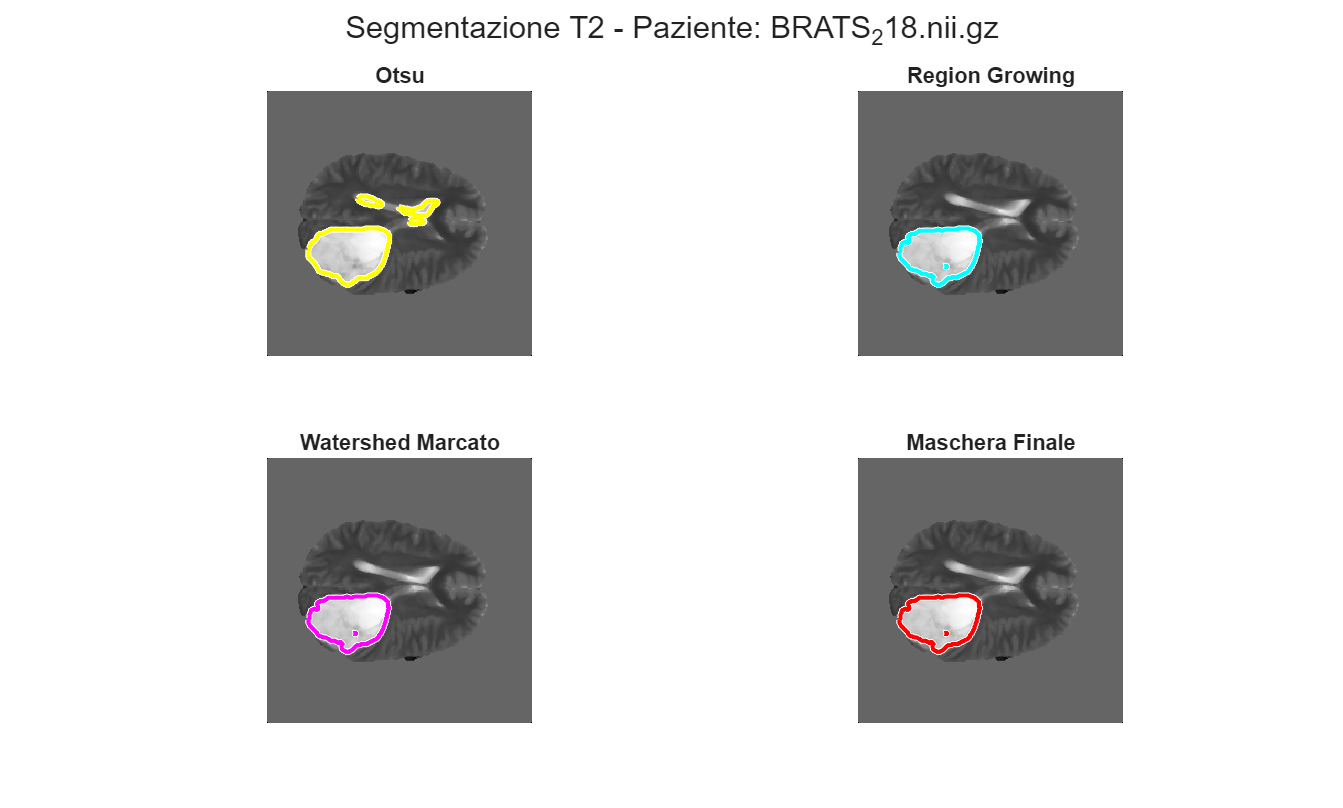
\includegraphics[width=\textwidth]{images/218_T2_segmentation.png}
    \caption{Risultati intermedi della segmentazione sulla sequenza \textit{T2}.}
    \label{fig:seg_t2}
\end{figure}

Per la sequenza \textit{T2} riportata in Figura~\ref{fig:seg_t2}, la sogliatura di Otsu riesce a individuare la regione tumorale, ma considera alcune aree secondarie errate.

\begin{figure}[H]
    \centering
    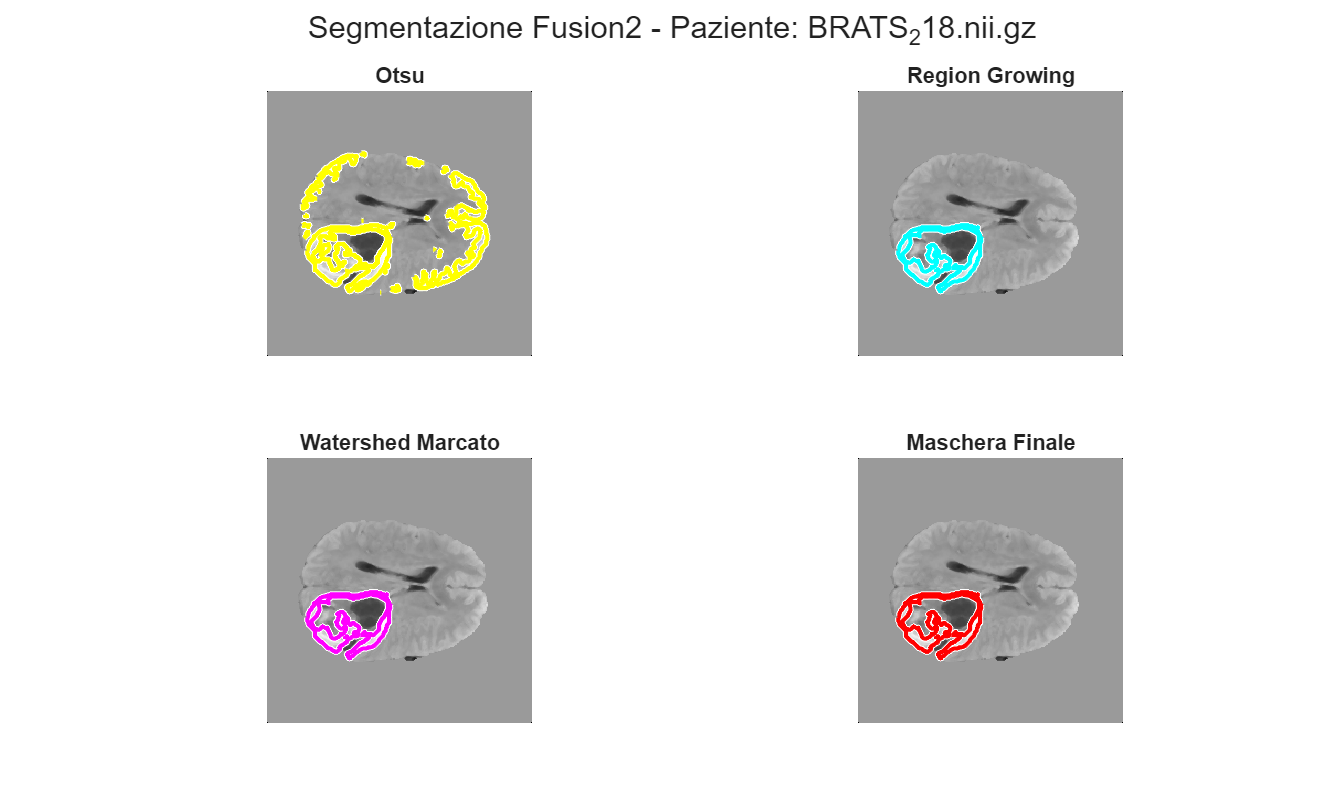
\includegraphics[width=\textwidth]{images/218_Fusion2_segmentation.png}
    \caption{Risultati intermedi della segmentazione sulla rappresentazione bimodale.}
    \label{fig:seg_fusion2}
\end{figure}

Nel caso della rappresentazione bimodale in Figura~\ref{fig:seg_fusion2}, la sogliatura di Otsu opera come nel caso precedente, sebbene in misura più contenuta rispetto alla sequenza \textit{FLAIR}.

\begin{figure}[H]
    \centering
    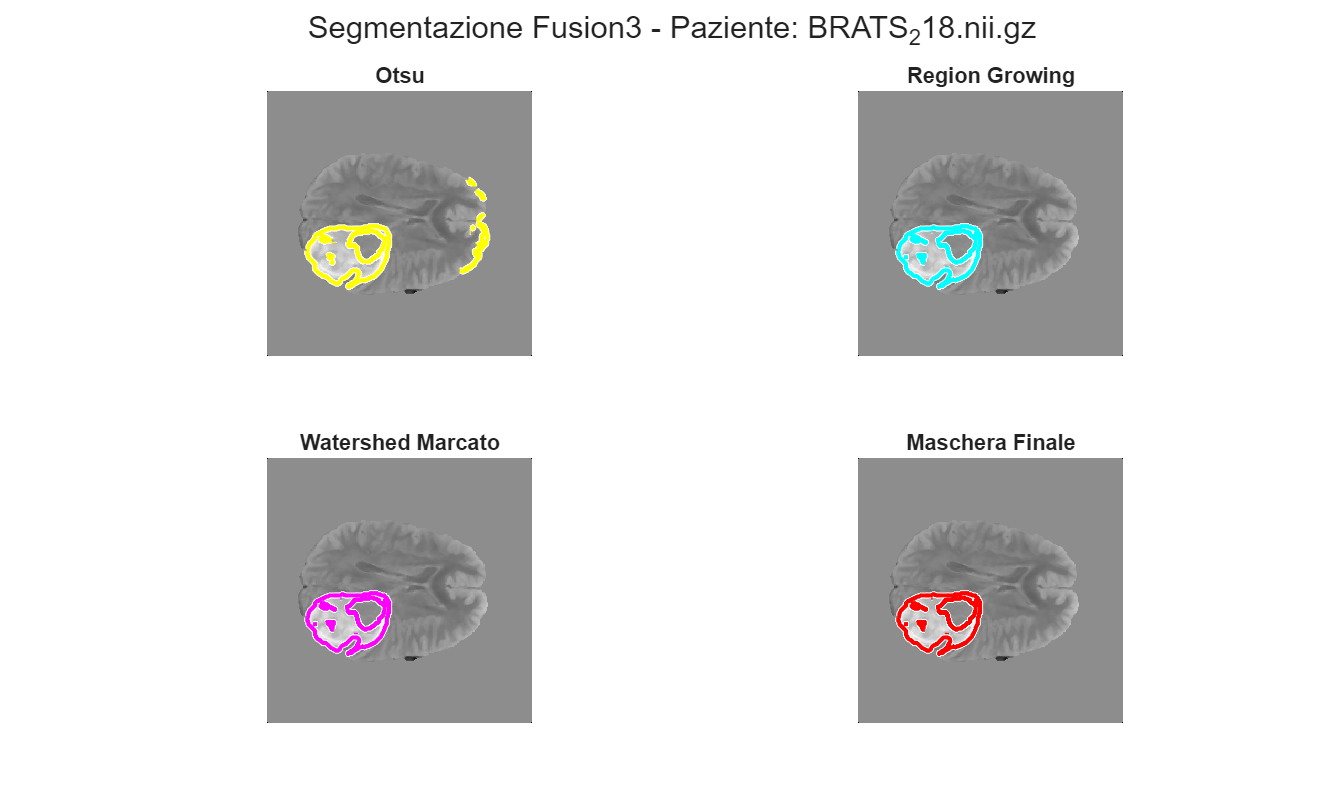
\includegraphics[width=\textwidth]{images/218_Fusion3_segmentation.png}
    \caption{Risultati intermedi della segmentazione sulla rappresentazione multimodale.}
    \label{fig:seg_fusion3}
\end{figure}

Nel caso della rappresentazione multimodale in Figura~\ref{fig:seg_fusion3}, la sogliatura iniziale di Otsu risulta già più selettiva rispetto alle altre configurazioni, concentrandosi maggiormente sulla regione tumorale rispetto alle zone periferiche.

Pertanto, tale maschera finale appare la più equilibrata tra estensione della lesione e regolarità del contorno grazie alla combinazione delle tre sequenze.

\subsection{Post-Processing}
La fase di post-processing rifinisce le maschere binarie ottenute dalla segmentazione, correggendo le irregolarità dei contorni e rimuovendo componenti residue. Le operazioni sono implementate nel modulo \textit{post\_processing.m}, che riceve in ingresso la maschera grezza, l’immagine preprocessata da utilizzare come sfondo per la visualizzazione, il nome della sequenza e l’identificativo del paziente.

Inizialmente, viene creata la cartella per il salvataggio dei risultati di post-processing per il paziente corrente. Successivamente, viene definito un elemento strutturante morfologico di forma circolare tramite la funzione \textit{strel("disk", 3)}.

\paragraph{Chiusura morfologica}
La prima operazione applicata alla maschera grezza è la chiusura morfologica con la funzione \textit{imclose}. La chiusura consiste in una dilatazione e un’erosione eseguite con lo stesso elemento strutturante.
Indicando con $M_{\text{raw}}$ la maschera binaria in ingresso e con $B$ l’elemento strutturante, la chiusura può essere espressa come:
\[
M_{\text{close}} = (M_{\text{raw}} \oplus B)\ominus B
\]
dove $\oplus$ indica la dilatazione e $\ominus$ l’erosione.

La dilatazione espande temporaneamente i contorni della regione segmentata, colmando piccole discontinuità, mentre l’erosione riduce la regione riportandola a dimensioni simili a quelle originali.

\paragraph{Riempimento delle cavità}
Dopo la chiusura morfologica, si applica la funzione \textit{imfill(mask\_clean, "holes")} per riempire le cavità interne alla maschera, ovvero le regioni di pixel di sfondo circondate da pixel appartenenti all’oggetto segmentato. Esse vengono convertite in pixel dell’oggetto senza modificare lo sfondo esterno alla maschera.

\paragraph{Selezione della componente connessa principale}
L’ultima operazione consiste nell’applicazione della funzione \textit{bwareafilt(mask\_clean, 1)}, che preserva la componente connessa di area maggiore (il parametro $1$ indica una sola componente).

La funzione analizza tutte le componenti connesse presenti nella maschera, calcola l’area in base al numero di pixel e seleziona soltanto quella più estesa.

\paragraph{Risultati grafici}
Per ogni configurazione, il modulo genera una figura di confronto tra la maschera grezza di segmentazione e la maschera finale dopo il post-processing. In entrambi i casi, il contorno della regione segmentata viene sovrapposto all’immagine preprocessata con la funzione \textit{visboundaries}.

Di seguito, si riportano i risultati nelle Figure~\ref{fig:post_flair}, \ref{fig:post_t1c}, \ref{fig:post_t2}, \ref{fig:post_fusion2} e \ref{fig:post_fusion3}.

\begin{figure}[H]
    \centering
    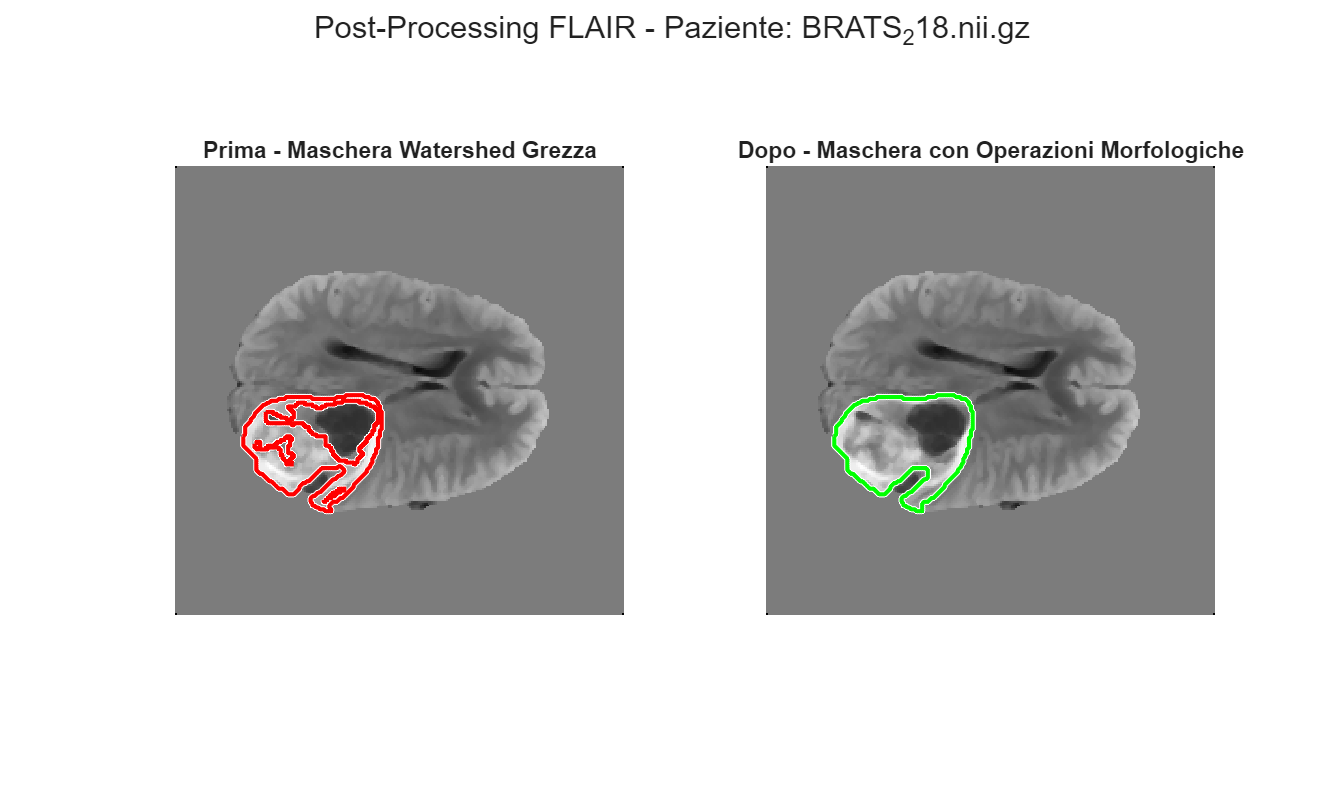
\includegraphics[width=\textwidth]{images/218_FLAIR_post_processing.png}
    \caption{Confronto tra maschera grezza e maschera raffinata dopo post-processing per la sequenza \textit{FLAIR}.}
    \label{fig:post_flair}
\end{figure}

\begin{figure}[H]
    \centering
    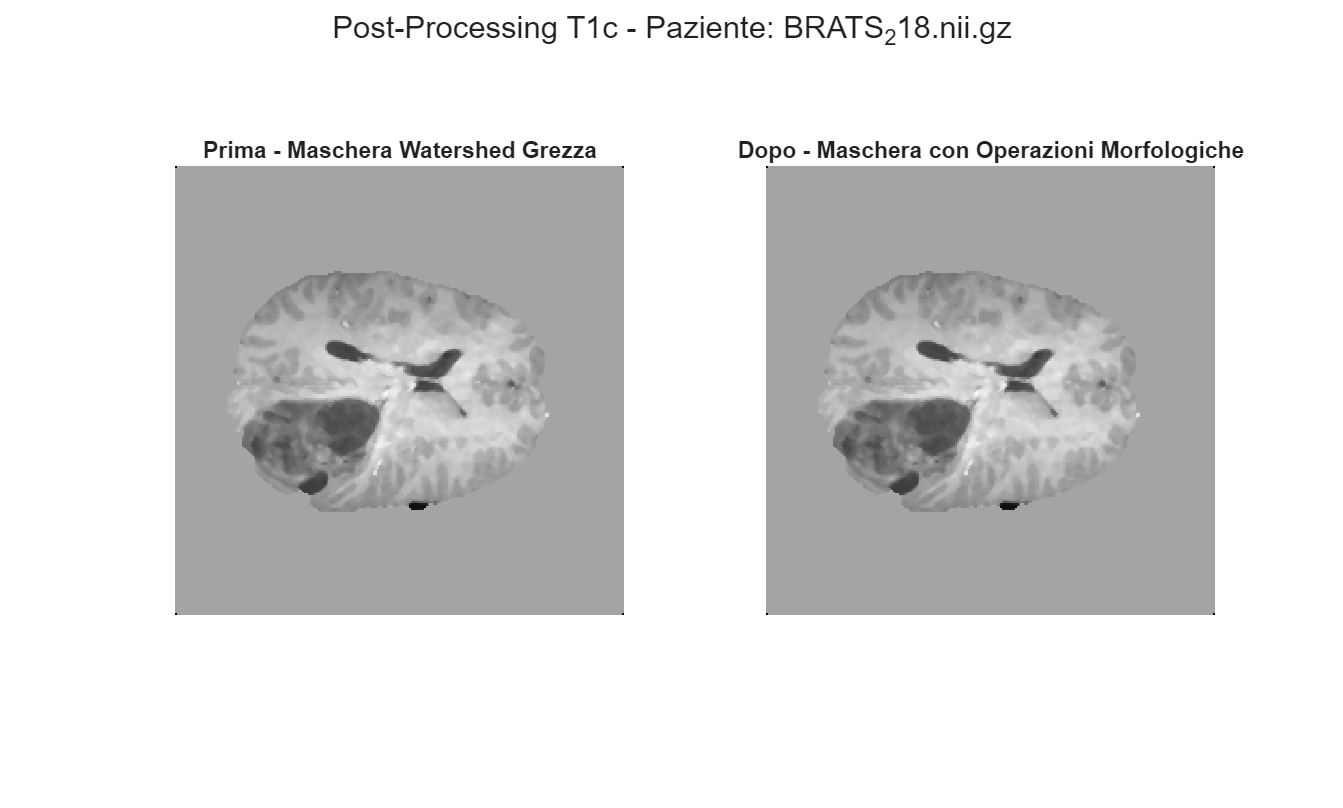
\includegraphics[width=\textwidth]{images/218_T1c_post_processing.png}
    \caption{Confronto tra maschera grezza e maschera raffinata dopo post-processing per la sequenza \textit{T1c}.}
    \label{fig:post_t1c}
\end{figure}

\begin{figure}[H]
    \centering
    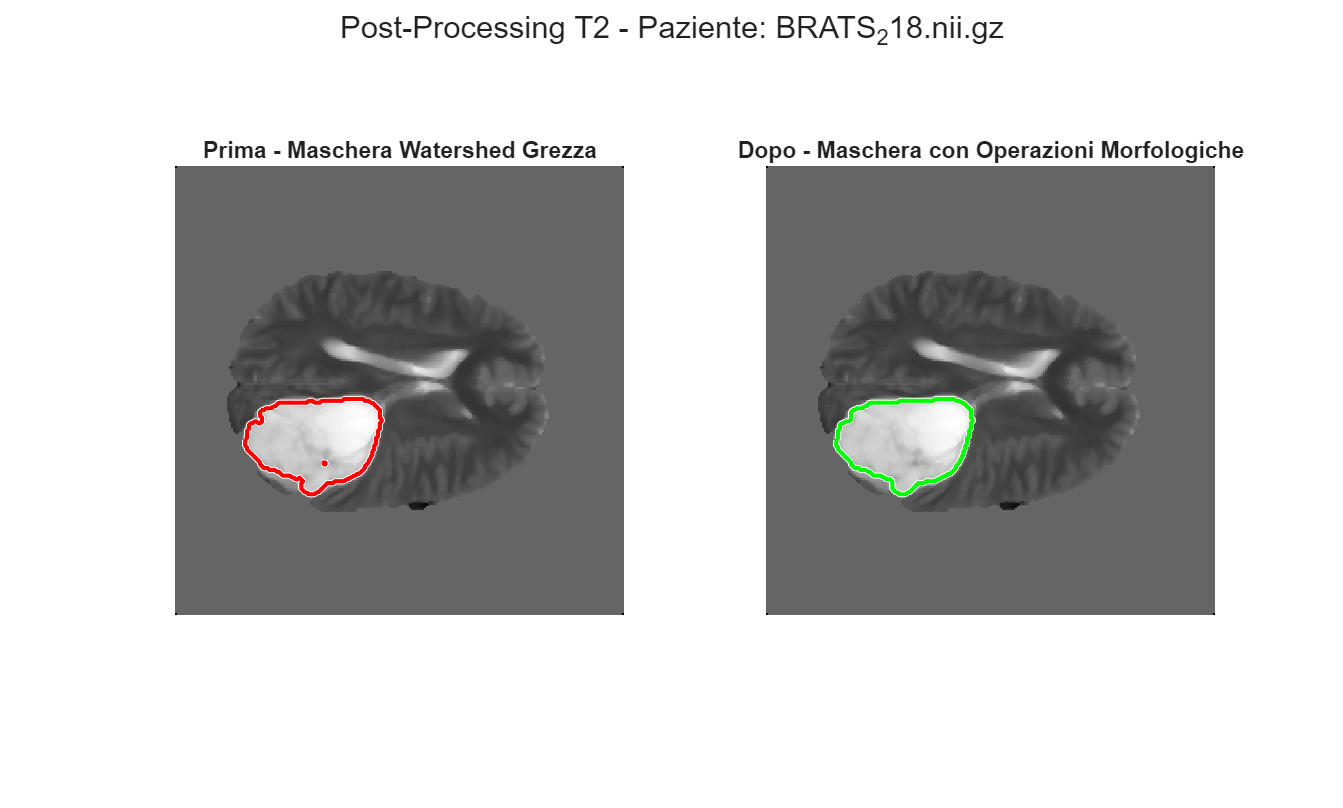
\includegraphics[width=\textwidth]{images/218_T2_post_processing.png}
    \caption{Confronto tra maschera grezza e maschera raffinata dopo post-processing per la sequenza \textit{T2}.}
    \label{fig:post_t2}
\end{figure}

\begin{figure}[H]
    \centering
    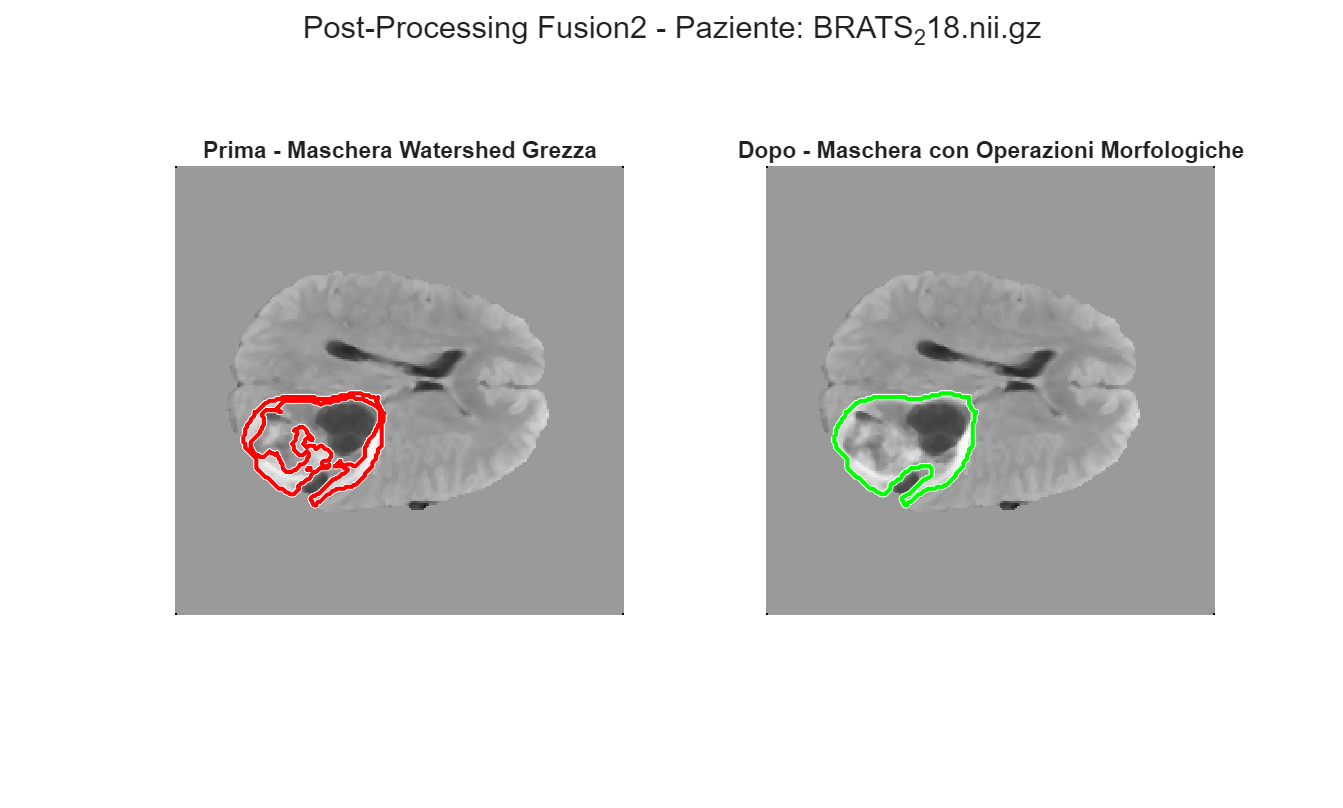
\includegraphics[width=\textwidth]{images/218_Fusion2_post_processing.png}
    \caption{Confronto tra maschera grezza e maschera raffinata dopo post-processing per la rappresentazione bimodale.}
    \label{fig:post_fusion2}
\end{figure}

\begin{figure}[H]
    \centering
    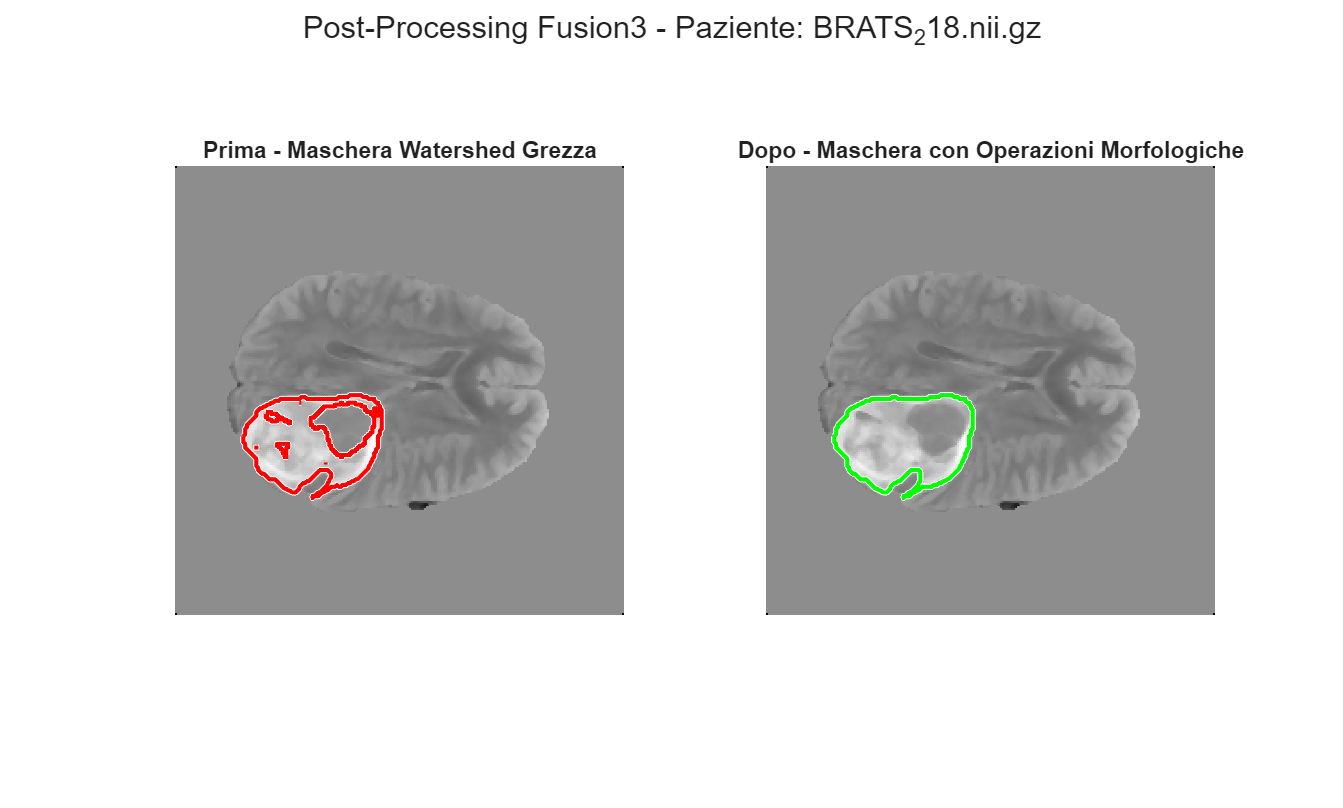
\includegraphics[width=\textwidth]{images/218_Fusion3_post_processing.png}
    \caption{Confronto tra maschera grezza e maschera raffinata dopo post-processing per la rappresentazione multimodale.}
    \label{fig:post_fusion3}
\end{figure}

Nelle configurazioni \textit{FLAIR}, \textit{Fusion2} e \textit{Fusion3} si osserva l'effettivo riempimento delle cavità interne e una maggiore continuità del bordo, mentre nella \textit{T2} l’intervento risulta più contenuto, poiché la maschera grezza appare già compatta. Nel caso della \textit{T1c}, invece, il post-processing non compensa l’assenza di una segmentazione efficace. 

\subsection{Valutazione}
L’ultima fase della pipeline riguarda la valutazione delle maschere di segmentazione ottenute. Tale operazione è implementata nella funzione \textit{evaluation.m}, che confronta la sovrapposizione della maschera binaria predetta con la corrispondente ground truth binaria.

Le metriche ottenute per i singoli pazienti e per l'intero dataset vengono memorizzate in due file CSV. In particolare, vengono calcolate tre metriche standard:

\begin{itemize}
    \item \textbf{Dice Score}: fornisce una misura complessiva della qualità della sovrapposizione, poiché tiene conto sia dei falsi positivi che dei falsi negativi;
    \item \textbf{Sensitivity}: evidenzia la capacità di recuperare la regione tumorale reale;
    \item \textbf{Precision}: misura il contenimento delle regioni spurie e dei falsi positivi.
\end{itemize}

La funzione riceve in ingresso due maschere binarie, corrispondenti alla segmentazione predetta dalla pipeline (\textit{mask\_pred}) e alla ground truth di riferimento (\textit{mask\_gt}). Entrambe le maschere vengono interpretate come immagini binarie della stessa dimensione, in cui i pixel appartenenti alla regione tumorale assumono valore logico vero, mentre i pixel di sfondo assumono valore falso.

Il primo passo consiste nel calcolo a livello di pixel di:
\begin{itemize}
    \item \textbf{True Positive (TP)}: pixel correttamente classificati come tumore;
    \item \textbf{False Positive (FP)}: pixel classificati come tumore dalla predizione, ma assenti nella ground truth;
    \item \textbf{False Negative (FN)}: pixel appartenenti alla ground truth tumorale, ma non rilevati dalla segmentazione.
\end{itemize}

Tali quantità vengono ottenute mediante operazioni logiche elemento per elemento tra le due maschere:
\[
TP = \sum \big(mask_{\text{pred}} \land mask_{\text{gt}}\big)
\]
\[
FP = \sum \big(mask_{\text{pred}} \land \neg mask_{\text{gt}}\big)
\]
\[
FN = \sum \big(\neg mask_{\text{pred}} \land mask_{\text{gt}}\big)
\]
dove il simbolo $\land$ indica l’operatore logico AND e $\neg$ la negazione logica.

\paragraph{Dice Score}
La prima metrica calcolata è il \textit{Dice Score}, che rappresenta una misura di similarità spaziale tra la segmentazione predetta e la ground truth. Esso è definito come:
\[
Dice = \frac{2TP}{2TP + FP + FN}.
\]

Il \textit{Dice Score} assume valori compresi tra 0 e 1. Un valore pari a 1 indica una sovrapposizione perfetta tra maschera predetta e ground truth, mentre un valore pari a 0 indica assenza totale di sovrapposizione.

\paragraph{Sensitivity}
La seconda metrica è la \textit{Sensitivity}, nota anche come \textit{Recall}, che misura la capacità dell’algoritmo di individuare correttamente i pixel tumorali realmente presenti nella ground truth:
\[
Sensitivity = \frac{TP}{TP + FN}
\]

Anche questa metrica varia tra 0 e 1. Un valore elevato indica che la pipeline riesce a rilevare gran parte della lesione, riducendo i falsi negativi. Un valore basso corrisponde alla mancata identificazione di porzioni tumorali effettivamente presenti.

\paragraph{Precision}
La terza metrica è la \textit{Precision}, che misura la quota di pixel classificati come tumore che risultano realmente corretti:
\[
Precision = \frac{TP}{TP + FP}
\]

Un valore elevato indica che la segmentazione introduce pochi falsi positivi, ovvero poche aree etichettate in modo errato.

L’uso congiunto di queste metriche consente un'interpretazione completa dei risultati della pipeline. Ad esempio, una segmentazione può ottenere una \textit{Sensitivity} elevata ma una \textit{Precision} bassa, indicando una buona capacità di individuare il tumore, ma con una maschera più estesa del necessario.
Viceversa, una \textit{Precision} elevata associata a una \textit{Sensitivity} ridotta suggerisce una segmentazione più selettiva, ma incapace di includere l’intera area della lesione.